\section{What the patents are worth}\label{sec:values}

Survival is a coarse measure: it ignores how much fees differ between offices and over a patent's life. Renewal
models turn each patent's fee path and lapse decision into money. Fees come from official schedules for each of the
ten offices by year of life and period, deflated to 2024 prices with each country's consumer price index and
converted at 2024 purchasing-power parities \citep{WDI}.

\paragraph{Two models.} In the deterministic model \citep{SchankermanPakes1986}, a patent earns $r_0 d^t$ in year $t$
after grant: $r_0$ is its return in the year of grant and $d$ the share of returns that carries over to the next
year, so returns decline at rate $1-d$. Initial returns are log-normal, $\ln r_0 \sim N(\alpha_g + \gamma \ln(1+n_i),
\sigma)$, where $n_i$ is the patent's forward citations, $\alpha_g$ the mean log return of owner group $g$
(domestic or foreign $\times$ firm size or university), $\gamma$ the elasticity of returns with respect to citations
and $\sigma$ the standard deviation of log returns. With returns falling and fees rising, the owner renews while
returns over the period a fee covers exceed the fee. In this model the rate of decline $1-d$ is not identified, so I also estimate the
learning model of \citet{Pakes1986}, in which log returns follow a random walk whose shocks shrink as owners learn,
and owners may keep a patent worth less than its fee for the option of later renewals. Where fees rise steeply every year $d$ is identified: 0.850 in Germany, 0.827 in the United Kingdom
and 0.831 in France, close to earlier renewal estimates, which put the decay of returns at 10--20 percent a
year \citep{SchankermanPakes1986,Griliches1990}; elsewhere the rate is not identified. I fix $d = 0.85$ everywhere. Appendix~\ref{app:models} sets out both models; Supplemental Appendix~S4 describes the fee schedules and reports the estimates.

\paragraph{Patent-level values.} Group averages could hide the patents that matter, and they depend on how owners are
grouped. I therefore value each patent from its own renewal history: the learning model is re-estimated with the same
starting distribution of returns for all owners, which depends only on citations, and each patent's value is the
median over simulated return paths, weighting each path by how likely it makes the patent's observed lapse or
survival. Owner type plays no
role in a patent's value. Figure~\ref{fig:valuespooled} compares, for each owner group, the values of domestic and
foreign owners' patents on the same fee path, in the same citation band and in the same field of the same office.\footnote{\label{fn:valuespecs}Each patent's posterior median value at grant from the learning model with a common prior ($d=0.85$; 2024 PPP dollars), regressed on domestic owner $\times$ owner group with fee-path $\times$ citation-band, office $\times$ field and office $\times$ owner-group effects; standard errors
clustered by owner; 1.17 million patents (Russia, and Brazilian patents granted before June 2009, left out). The emerging-minus-advanced difference is an interaction in one regression.}
This is the home premium.

\begin{figure}[!htbp]
\centering
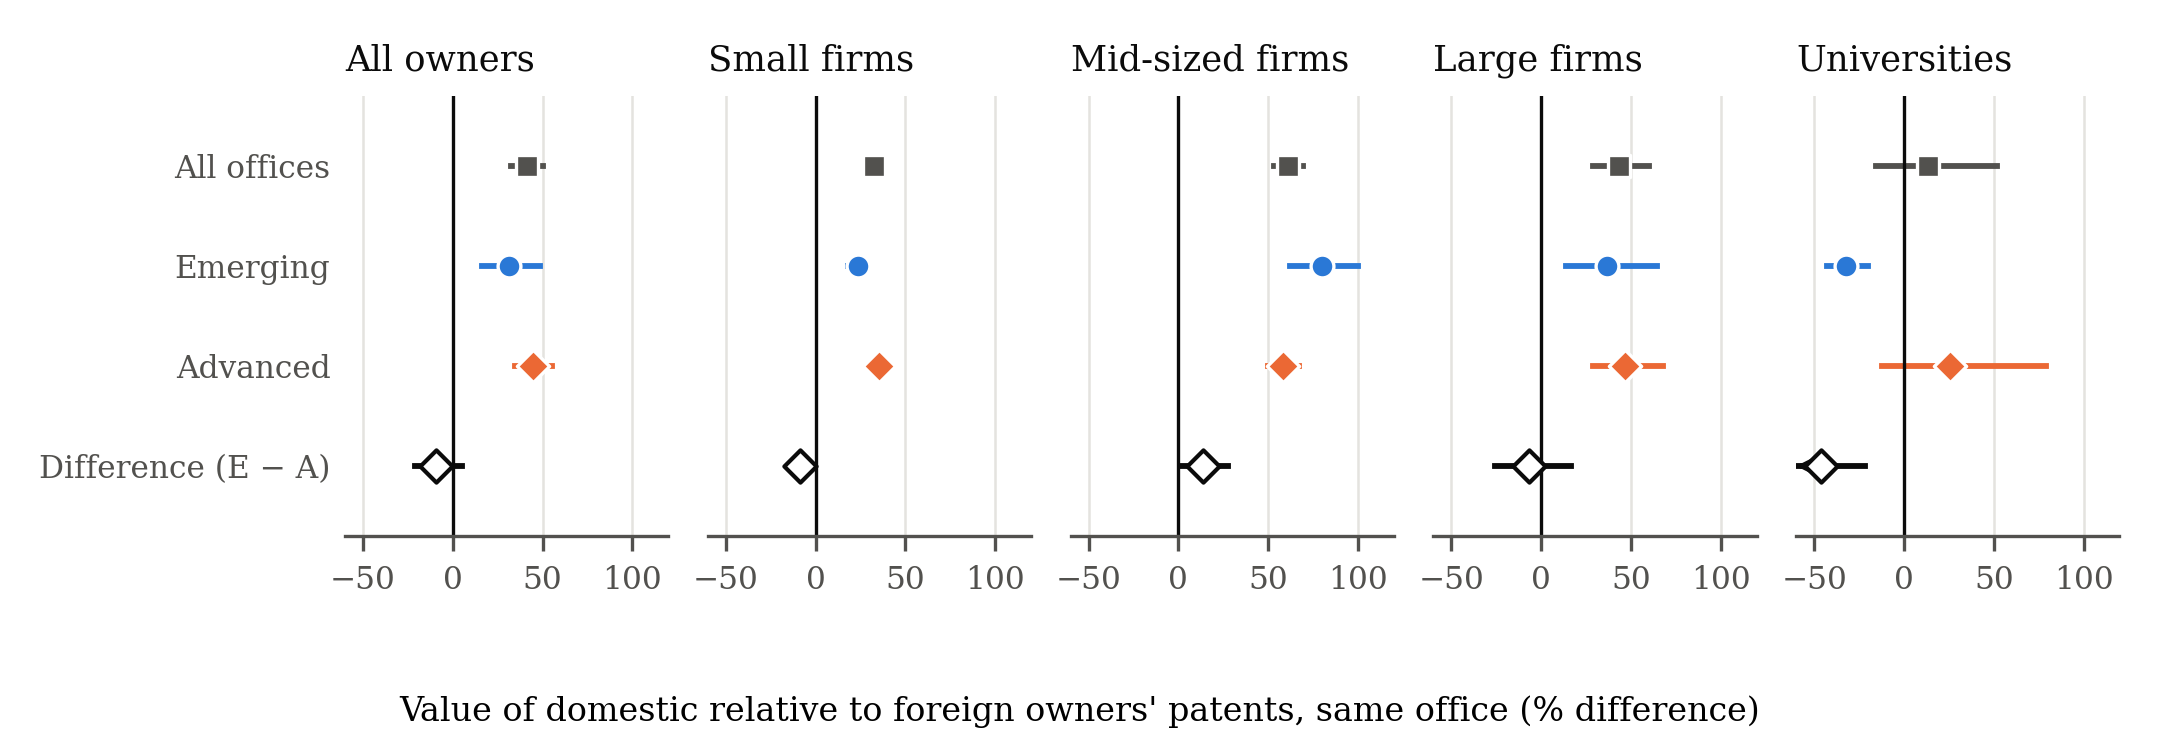
\includegraphics[width=\textwidth]{figures/fig7_values_pooled.png}
\caption{Value of domestic relative to foreign owners' patents, by owner group}\label{fig:valuespooled}
\figurenotes{Point estimates with 95\% confidence intervals, in percent, $100(e^{b}-1)$ for a log-value gap $b$; for the difference, the percentage by which the emerging-market ratio exceeds the advanced one.
Squares: all offices; circles: emerging-market offices (Russia left out, its values not identified); diamonds:
advanced-economy offices; open diamonds: emerging minus advanced. Value: each patent's value at grant estimated from its
own renewal history. Specification in footnote~\ref{fn:valuespecs}.}
\end{figure}

\paragraph{The home premium.} Domestic owners value their patents more than foreign owners in the same office, as
they should: the home market is where they sell. Across all owners the premium is smaller in the emerging-market offices, but not significantly: domestic owners'
patents are worth 31\% more than foreign owners' there\footnote{\label{fn:russia}Russia is left out:
its values are not identified. Domestic owners paid very low fees, about \$50--150 a year in PPP terms, but let many
patents lapse, while foreign owners paid four and a half times the resident fee until 2012 and kept theirs; the model
cannot separate low value from lapses unrelated to the fee.} and 45\% more
in the advanced ones. For mid-sized firms it is larger in the emerging-market offices, 80\% against 58\%; for large
firms it is 37\% against 47\%, not significantly different. Small firms' home premium is 23\% in the
emerging-market offices and 35\% in the advanced ones, 9\% less. As in Section~\ref{sec:survival}, the benchmark matters. Small
Japanese firms value their home patents far above foreign owners do in Japan (226\% more), and Japan contributes a
large share of the advanced-economy patents. Office by office, the premium of small firms is 29\% in China and
65\% in Korea, against 28\% in the United States, 31\% in Germany and 8\% in the United Kingdom; it is 7\% in Brazil,
imprecisely, and close to zero in the Czech Republic and France (Supplemental Appendix Table~S8). Universities are the exception among
emerging-market owners: Chinese universities' patents are worth 59\% less than foreign universities' patents in China
($1-e^{-0.88}$). The deterministic model and other decay rates give the same pattern (Supplemental Appendix~S4).

\paragraph{Fee discounts do not change the comparison.} China and Korea cut renewal fees for domestic small firms and
universities (as does Brazil), and the models above assume standard fees. Lower fees mean the same renewal behaviour implies lower
values, so I re-estimate both models for China and Korea assuming that every eligible owner took the discount: in China, 30\% of the fee
in the first three fee-years after grant until 2016, then 15\% for six fee-years and, from 2018, for ten; in Korea, 70\% of the fee
in years 4--6 from 2014 and half from 2018. The ratio of small domestic to
small foreign firms' median value at equal citations barely moves: from 2.04 to 1.99 in China and from 2.72 to 2.63 in
Korea in the deterministic model, and from 1.95 to 1.98 and from 2.31 to 2.08 in the learning model. 

\paragraph{Levels are rough; comparisons are not.} A typical small domestic firm's patent is worth roughly
\$5{,}000--62{,}000 at grant in the deterministic model and more, in some offices several times more, in the learning model, in which early
lapses reflect learning rather than low initial value. Values in different offices also cover protection in
different markets. The comparisons between owners, on which the argument rests, are stable across models, decay rates
and fee assumptions, except in Russia. Because a patent's value on a given fee path rises with how long it is kept,
the patent-level values restate the survival results in money.
